% Name: Communication system
% Description: Transmitter, noisy channel, and receiver, with each side grouped in a dashed box.
% Tags: communication, channel, signal processing

\usetikzlibrary{arrows.meta, positioning, fit}

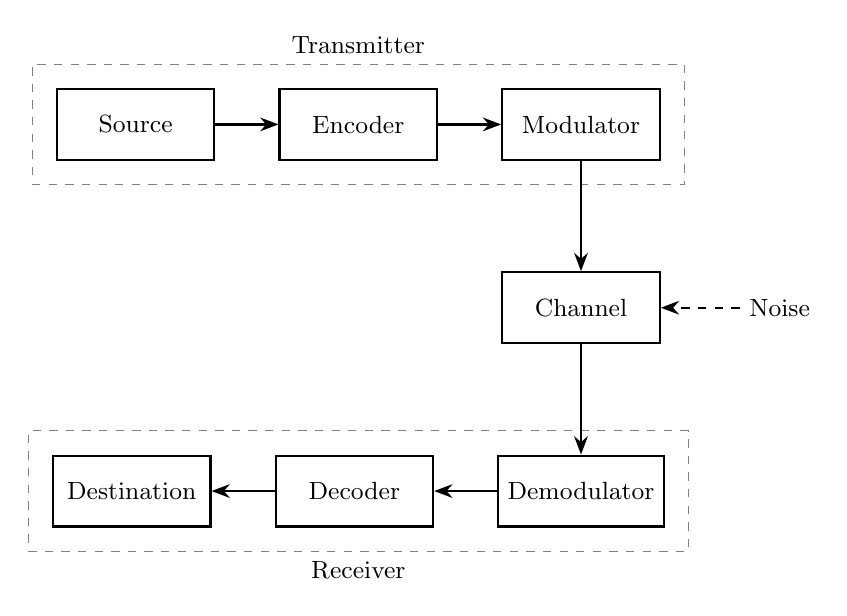
\begin{tikzpicture}[
  node distance=6mm and 8mm,
  every node/.style={font=\small},
  block/.style={draw, thick, minimum height=9mm, minimum width=20mm},
  group/.style={draw, dashed, gray, inner sep=3mm},
  arrow/.style={-{Stealth}, thick},
]
  \node[block] (src) {Source};
  \node[block, right=of src] (enc) {Encoder};
  \node[block, right=of enc] (mod) {Modulator};
  \node[block, below=14mm of mod] (ch) {Channel};
  \node[block, below=14mm of ch] (dem) {Demodulator};
  \node[block, left=of dem] (dec) {Decoder};
  \node[block, left=of dec] (sink) {Destination};
  \node[right=10mm of ch] (noise) {Noise};

  \node[group, fit=(src)(mod), label=above:Transmitter] {};
  \node[group, fit=(sink)(dem), label=below:Receiver] {};

  \draw[arrow] (src) -- (enc);
  \draw[arrow] (enc) -- (mod);
  \draw[arrow] (mod) -- (ch);
  \draw[arrow] (ch) -- (dem);
  \draw[arrow] (dem) -- (dec);
  \draw[arrow] (dec) -- (sink);
  \draw[arrow, dashed] (noise) -- (ch);
\end{tikzpicture}
